% Provenance (never printed): see sources/outline_sources.md (Year 3: rift
% models, normal-fault systems, metamorphic core complexes, strike-slip
% systems). Brief: sources/book5/BRIEFS.md, ch. 9. Curves from
% figdata/bachelor-3/domino_extension.py and rollover.py. Exercise and problem
% values in the Book 5 scratch calculator calc/ch09.py.
\chapter{التكتونية الاستطالية والانزياحية}\label{ch:b3:extension-strike-slip}

بين سييرا نيفادا وهضبة كولورادو تتعاقب السلاسل الجبلية والأحواض
تتناوب كأخاديد الحقل، إذ تمثّل كل سلسلة كتلةً من القشرة مائلةً على طول صدع عادي
وفي لبّ بعض هذه السلاسل تقع صخور كانت مدفونة
مدفونةً على عمق بين 23 و\qty{30}{km}، وعند درجة حرارة من 500 إلى \qty{650}{\celsius}، تقع اليوم عند
السطح، تحت صدع واحد لا يتجاوز انحداره بضع درجات.
يمكن أن تُمَدَّد القارة بعامل يساوي اثنين أو أكثر، وأن تتمزّق جانبيًا على طول صدوع
تنحني وتتدرّج وتفتح أحواضًا يبلغ عمقها \qty{10}{km}. يبني هذا الفصل
هندسة الاستطالة والصدع الانزياحي، والقواعد القليلة التي
تحكمه، والشواهد التي تتركها الأنظمة الحقيقية.
% ledger: cooper10:snake-range, mcq05:basin-range, tb93:dead-sea-basin

\begin{recall}
الصدوع العادية والانزياحية والتحويلية، ونصف الغرابن والشقّ القاري
ترد في مجلد السنة الأولى، في فصليه عن الشقوق، وعن الصدوع والطيات
والأنسجة الصخرية، مع نظرية أندرسون: عندما يكون $\sigma_1$ شاقوليًا، تميل الصدوع العادية
بزاوية $\ang{45} + \phi/2$، أي نحو \ang{60}؛ وعندما يكون $\sigma_2$ شاقوليًا، تمتدّ الصدوع الانزياحية
بزاوية $\ang{45} - \phi/2$ عن $\sigma_1$. وقانون بيرلي لاحتكاك الصخور،
$\tau = 0.85\,\sigma_n$ تحت \qty{200}{MPa}، و$\tau =
\qty{50}{MPa} + 0.6\,\sigma_n$ فوق ذلك، وهو وارد في فصله عن الإجهاد والانفعال
والريولوجيا. أمّا نموذج الاستطالة، الذي يُرقَّق فيه الغلاف الصخري بانتظام
بمقدار عامل $\beta$، وحوض الشقّ، فيرد كلاهما في مجلد السنة الثانية، في فصله
المقارن بين الأحواض الرسوبية. وترد نطاقات القصّ والميلونيت في
\cref{ch:b3:deformation-mechanisms}؛ أمّا عمق الانفصال انطلاقًا من المساحة الفائضة
$A = Sh$، فيرد في \cref{ch:b3:structural-analysis}.
\end{recall}
% ledger: byerlee:1975

\section{نموذجان للشقّ}\label{sec:b3:extension-strike-slip:models}

يُرقّق نموذج الاستطالة الوارد في مجلد السنة الثانية الغلاف الصخري كلّه بالعامل
نفسه تحت الموقع نفسه: فتترقّق القشرة والوشاح معًا،
بشكل متماثل، بالقصّ الخالص. وكثير من الحواف المتشقّقة غير متماثل: فأحد جانبيه
هو منطقة واسعة من الكتل المائلة، والآخر منحدر ضيّق شديد،
ويقع ترقّق الوشاح بجانب ترقّق القشرة لا تحته.

\begin{definition}[نموذج التصدّع بالقصّ البسيط]\label{def:b3:extension-strike-slip:rift-models}
في \emph{نموذج التصدّع بالقصّ البسيط}\index{نموذج التصدّع بالقصّ البسيط} يُشدّ
الغلاف الصخري على طول نطاق قصّ منخفض الزاوية يقطعه من
السطح حتى قاعدته. وتفقد الصفيحة الواقعة فوق \omterm{def:b3:deformation-mechanisms:shear-zone}{نطاق القصّ}، أي الصفيحة العليا،
جزءها السفلي؛ أمّا الصفيحة الواقعة تحته، أي الصفيحة السفلى، فتُسحب
من تحتها. ويكون ترقّق القشرة وترقّق الوشاح
متزحزحين جانبيًا، والحافتان المترافقتان اللتان تنشآن حين تنفصل القارة
فتكونان غير متماثلتين.
\end{definition}

تجمع الشقوق الحقيقية بين النموذجين: تصدّعٌ هشّ في القشرة العليا، وترقّقٌ لدنٌ
تحتها، ووشاح قد يترقّق على منطقة أوسع أو أضيق من
القشرة (استطالة تعتمد على العمق). حيث يصعد الوشاح الساخن تحت
الشقّ، أو تحت جانبه في حالة القصّ البسيط، يرفع الطفو
كتفي الشقّ، فتقف جبالًا فوق قاع الحوض.

\begin{omfigure}
\begin{tikzpicture}[scale=0.95, >=stealth]
% (a) pure shear
\begin{scope}
\fill[omLithBasalt!40] (0,-3.2) rectangle (6.6,-1.3);
\fill[omLithGranite!50] (0,0) -- (2.2,0) -- (2.5,-0.35) -- (4.1,-0.35) -- (4.4,0) -- (6.6,0) -- (6.6,-1.3)
  -- (4.4,-1.3) -- (3.3,-0.95) -- (2.2,-1.3) -- (0,-1.3) -- cycle;
\fill[omLithBasalt!40] (2.2,-1.3) -- (3.3,-0.95) -- (4.4,-1.3) -- cycle;
\fill[orange!25] (0,-3.2) -- (1.8,-3.2) -- (3.3,-2.1) -- (4.8,-3.2) -- (6.6,-3.2) -- (6.6,-3.7) -- (0,-3.7) -- cycle;
\draw (0,0) -- (2.2,0) -- (2.5,-0.35) -- (4.1,-0.35) -- (4.4,0) -- (6.6,0);
\draw (0,-1.3) -- (2.2,-1.3) -- (3.3,-0.95) -- (4.4,-1.3) -- (6.6,-1.3);
\draw (0,-3.2) -- (1.8,-3.2) -- (3.3,-2.1) -- (4.8,-3.2) -- (6.6,-3.2);
\draw[thick] (2.2,0) -- (2.75,-0.85); \draw[thick] (4.4,0) -- (3.85,-0.85);
\node[font=\scriptsize] at (0.7,-0.65) {القشرة};
\node[font=\scriptsize, align=center] at (0.9,-2.25) {الغلاف الصخري\\ الوشاحي};
\node[font=\scriptsize] at (1.2,-3.48) {الغلاف اللدن};
\draw[<-] (-0.1,0.25) -- (0.6,0.25); \draw[->] (6.0,0.25) -- (6.7,0.25);
\node[font=\small] at (3.3,-4.2) {\foreignlanguage{arabic}{(أ) القصّ الخالص}};
\end{scope}
% (b) simple shear: crust thinned near the breakaway (left), mantle beneath the upper plate (right)
\begin{scope}[xshift=7.4cm]
\fill[omLithBasalt!40] (0,-3.2) rectangle (6.6,-1.3);
\fill[omLithGranite!50] (0,0) -- (0.9,0) -- (1.2,-0.3) -- (2.2,-0.3) -- (2.5,0) -- (4.0,0)
  .. controls (4.6,0.18) and (5.2,0.18) .. (5.8,0) -- (6.6,0) -- (6.6,-1.3)
  -- (2.9,-1.3) -- (2.0,-0.7) -- (1.2,-1.3) -- (0,-1.3) -- cycle;
\fill[omLithBasalt!40] (1.2,-1.3) -- (2.0,-0.7) -- (2.9,-1.3) -- cycle;
\fill[orange!25] (0,-3.2) -- (3.4,-3.2) -- (4.8,-2.1) -- (6.0,-3.2) -- (6.6,-3.2) -- (6.6,-3.7) -- (0,-3.7) -- cycle;
\draw (0,0) -- (0.9,0) -- (1.2,-0.3) -- (2.2,-0.3) -- (2.5,0) -- (4.0,0)
  .. controls (4.6,0.18) and (5.2,0.18) .. (5.8,0) -- (6.6,0);
\draw (0,-1.3) -- (1.2,-1.3) -- (2.0,-0.7) -- (2.9,-1.3) -- (6.6,-1.3);
\draw (0,-3.2) -- (3.4,-3.2) -- (4.8,-2.1) -- (6.0,-3.2) -- (6.6,-3.2);
\draw[omThm, very thick] (0.9,0) .. controls (2.4,-0.9) and (3.9,-1.8) .. (5.4,-3.2);
\node[font=\scriptsize, align=center] at (5.0,-0.6) {الصفيحة العليا};
\node[font=\scriptsize, align=center] at (1.3,-2.3) {الصفيحة السفلى};
\node[omThm, font=\scriptsize, align=center] at (3.0,-2.15) {نطاق\\ القصّ};
\node[font=\scriptsize, align=center] at (4.9,0.42) {الجانب المرتفع};
\draw[<-] (-0.1,0.25) -- (0.6,0.25); \draw[->] (6.0,0.25) -- (6.7,0.25);
\node[font=\small] at (3.3,-4.2) {\foreignlanguage{arabic}{(ب) القصّ البسيط}};
\end{scope}
\end{tikzpicture}

\par\smallskip{\small نموذجان طرفيان للشقّ (غير مرسومين بالمقياس). (أ) القصّ الخالص:
تترقّق القشرة والغلاف الصخري الوشاحي معًا تحت الشقّ، مع
صدوع عادية على الجانبين. (ب) القصّ البسيط: نطاق قصّ منخفض الزاوية يعبر
الغلاف الصخري؛ فتترقّق القشرة قرب أثره على السطح، ويترقّق الوشاح تحت
الجانب البعيد، تحت الصفيحة العليا، فيغدو الشقّ غير متماثل،
وجانبه فوق الوشاح المترقّق يرتفع.}\label{fig:b3:extension-strike-slip:models}
\end{omfigure}

\section{أنظمة الصدوع العادية}\label{sec:b3:extension-strike-slip:faults}

\begin{definition}[التصدّع الدومينوي]\label{def:b3:extension-strike-slip:domino}
في \emph{التصدّع الدومينوي}\index{التصدّع الدومينوي} تقطع مجموعة من الصدوع العادية المستوية المتوازية
القشرة العليا إلى كتل صلبة، تدور معًا مع امتداد المنطقة
كصفّ من الكتب المتساقطة، فتصير الصدوع أقلّ انحدارًا،
ووالطبقات التي كانت أفقية في الأصل تميل في الاتجاه المعاكس.
\end{definition}

\begin{theorem}[الاستطالة بالدومينو]\label{thm:b3:extension-strike-slip:domino}
لتكن كتل صلبة محصورة بصدوع مستوية متوازية كان انحدارها في الأصل
$\theta_0$ تدور حتى يصير انحدار الصدوع $\theta$. ثم تنحدر الطبقات بمقدار $\theta_0
- \theta$ بعيدًا عن الصدوع، وقد استطالت المنطقة بالعامل
الآتي:
\[
  \beta = \frac{\sin\theta_0}{\sin\theta} .
\]
\end{theorem}

\begin{proof}
لأنّ الكتل صلبة، فإنّ المسافة العمودية $d$ بين صدعين
متجاورين لا تتغيّر. وعلى خطّ أفقي، يقطع مستويان متوازيان ينحدران بمقدار
$\theta$ ويبعد أحدهما عن الآخر $d$ قطعةً طولها $d/\sin
\theta$. ويتناسب عرض المنطقة طرديًا مع طول تلك القطعة، فيتغيّر من
$d/\sin\theta_0$ إلى $d/\sin\theta$. وتدور الكتل بالزاوية التي
تفلطحت بها الصدوع، أي $\theta_0 - \theta$، وتدور معها الطبقات
التي كانت أفقية في البداية.
\end{proof}

يعطي الدوران وحده استطالةً متواضعة: الصدوع التي تبدأ عند \ang{60}
وتتفلطح إلى \ang{30}، فتستطيل المنطقة بالعامل $\beta = 1.73$. ولا يمكنها أن تدور
إلى الأبد: يصعب انزلاق الصدع كلما تفلطح، لأنّ $\sigma_1$ الرأسي
يضغط عليه أكثر ويقصّه أقلّ.

\begin{proposition}[الانغلاق الاحتكاكي لصدع عادي]\label{prop:b3:extension-strike-slip:lockup}
ليكن صدعٌ عديم التماسك معامل احتكاكه $\mu$ يصنع الزاوية
$t$ مع $\sigma_1$، وتكون الإجهادات كلّها فعّالة. ينزلق الصدع حين تبلغ نسبة
الإجهادات الرئيسية القيمة الآتية:
\[
  \frac{\sigma_1}{\sigma_3} = \frac{1 + \mu\cot t}{1 - \mu\tan t} ,
\]
وهي أدنى قيمة، وتساوي $(\sqrt{1 + \mu^2} + \mu)^2$، عند $\tan2t = 1/\mu$، وتصير
لا نهائية عند $\tan t = 1/\mu$. ومع كون $\sigma_1$ رأسيًا، يكون انحدار الصدع
$\ang{90} - t$: فالصدع العادي الذي ينحدر بأقلّ من $\arctan\mu$ لا ينزلق
البتّة.
\end{proposition}

\begin{proof}
لنكتب $m = (\sigma_1 + \sigma_3)/2$ و$s = (\sigma_1 - \sigma_3)/2$. على
المستوى: $\sigma_n = \sigma_1\sin^2t + \sigma_3\cos^2t = m - s\cos2t$،
و$\tau = (\sigma_1 - \sigma_3)\sin t\cos t = s\sin2t$. ويشترط الانزلاق أن يكون $\tau =
\mu\sigma_n$؛ بقسمة الطرفين على $\sigma_3\sin t\cos t$ وجمع حدود $\sigma_1$
نحصل على النسبة، التي يتلاشى مقامها عند $\tan t = 1/\mu$. وفي الصيغة
الأخرى يُكتب الشرط $s(\sin2t + \mu\cos2t) = \mu m$. وأكبر ما يكون القوس
هو $\sqrt{1 + \mu^2}$، ويبلغ ذلك عند $\tan2t = 1/\mu$، حيث يشترط الانزلاق أدنى
قيمة للنسبة $s/m = \mu/\sqrt{1 + \mu^2}$؛ ومنه $\sigma_1/\sigma_3 = (m + s)/(m - s) =
(\sqrt{1 + \mu^2} + \mu)/(\sqrt{1 + \mu^2} - \mu) = (\sqrt{1 + \mu^2} +
\mu)^2$، لأنّ حاصل ضرب القوسين الأخيرين يساوي 1.
\end{proof}

مع معامل بيرلي $\mu = 0.6$، ينحدر الصدع العادي الأفضل توجّهًا بمقدار \ang{60.5}
وينزلق عندما يكون $\sigma_1 = 3.12\,\sigma_3$، ويحتاج الصدع عند \ang{45} إلى $4.0$،
ولا ينزلق أيّ صدع انحداره أقلّ من \ang{31}؛ ومع $\mu = 0.85$ يكون انحدار الانغلاق
\ang{40}. يبيّن الشكل أدناه النتيجتين. عندما تقترب مجموعة الدومينو
من الانغلاق، تقطع المجموعةَ القديمةَ مجموعةٌ جديدة من الصدوع الشديدة الانحدار:
فالمناطق الممتدّة بشدّة تُظهر عدّة أجيال من الصدوع.

\begin{omfigure}
\begin{tikzpicture}
\begin{groupplot}[group style={group size=2 by 1, horizontal sep=1.6cm},
  omrecord, width=0.47\linewidth, height=0.42\linewidth, title style={font=\small},
  legend style={font=\scriptsize, legend cell align=left}]
\nextgroupplot[title={(أ) الاستطالة بالدومينو الصلبة}, xlabel={انحدار الصدع الحالي $\theta$ \babelsublr{(\unit{\degree})}},
  ylabel={عامل الاستطالة $\beta$}, xmin=10, xmax=70, ymin=1, ymax=4,
  legend style={at={(0.97,0.97)}, anchor=north east}]
% computed in figdata/bachelor-3/domino_extension.py
\addplot[omDef, thick] table[x=dip, y=b70] {figdata/out/bachelor-3-domino_extension-beta.dat};
\addlegendentry{$\theta_0 = \ang{70}$}
\addplot[red!70!black, thick, densely dashed] table[x=dip, y=b60] {figdata/out/bachelor-3-domino_extension-beta.dat};
\addlegendentry{$\theta_0 = \ang{60}$}
\addplot[black, thick, densely dotted] table[x=dip, y=b45] {figdata/out/bachelor-3-domino_extension-beta.dat};
\addlegendentry{$\theta_0 = \ang{45}$}
\nextgroupplot[title={(ب) نسبة الإجهاد اللازمة للانزلاق}, xlabel={انحدار الصدع \babelsublr{(\unit{\degree})}},
  ylabel={$\sigma_1/\sigma_3$}, xmin=20, xmax=90, ymode=log, ymin=1, ymax=40,
  log ticks with fixed point, ytick={1,2,5,10,20,40},
  legend style={at={(0.97,0.97)}, anchor=north east}]
\addplot[omDef, thick] table[x=dip, y=r060] {figdata/out/bachelor-3-domino_extension-lockup.dat};
\addlegendentry{$\mu = 0.6$}
\addplot[red!70!black, thick, densely dashed] table[x=dip, y=r085] {figdata/out/bachelor-3-domino_extension-lockup.dat};
\addlegendentry{$\mu = 0.85$}
\end{groupplot}
\end{tikzpicture}

\par\smallskip{\small (أ) عامل الاستطالة لنطاق من الدومينو الصلب مع دوران
صدوعه من الانحدار الابتدائي $\theta_0$ إلى $\theta$. (ب) نسبة الإجهادات الرئيسية الفعّالة
اللازمة لانزلاق صدع عادي بانحدار معيّن
تحت $\sigma_1$ رأسي، لمعاملَي الاحتكاك عند بيرلي، وتبلغ أدنى قيمة
قرب \ang{60} و\ang{65}، وتصير لانهائية عند انحداري الانغلاق \ang{31}
و\ang{40}.}\label{fig:b3:extension-strike-slip:domino}
\end{omfigure}

تكون كثير من الصدوع العادية الكبيرة منحنية، شديدة الانحدار عند السطح، وتتفلطح
في العمق لتصير صدعًا أو نطاق قصّ شبه أفقي.

\begin{definition}[صدع الانفصال، الصدع اللستري، الطية المحدبة الانقلابية]\label{def:b3:extension-strike-slip:detachment}
\emph{صدع الانفصال}\index{صدع الانفصال} هو صدع عادي منخفض الانحدار
أو نطاق قصّ ذو إزاحة كبيرة، تُقاس بالكيلومترات إلى عشرات الكيلومترات، يفصل
صفيحة علوية ممتدّة عن صفيحة سفلية متشوّهة بشكل مختلف.
\emph{الصدع اللستري}\index{الصدع اللستري} صدع عادي يتناقص انحداره مع العمق،
ويكون مقطعه مقعّرًا نحو الأعلى. وحين يتحرّك الجدار المعلّق لصدع لستري
نحو الأسفل وبعيدًا، ينحني ليبقى على تماسّ مع الصدع:
فتميل طبقاته نحو الصدع في طيّة عريضة، هي \emph{الطية المحدبة
الانقلابية}\index{الطية المحدبة الانقلابية}.
\end{definition}

\begin{method}[بناء الإزاحة الأفقية الثابتة]\label{met:b3:extension-strike-slip:heave}
لرسم الجدار المعلّق لصدع لستري بعد إزاحة أفقية مقدارها
$H$، أي الإزاحة الأفقية، على مقطع موازٍ للانزلاق:
\begin{enumerate}
  \item نقسّم الجدار المعلّق إلى أعمدة رأسية. نُزيح كلّ عمود جانبيًا
        بمقدار $H$، بعيدًا عن الجدار المرتكز.
  \item نُنزل كلّ عمود بمقدار هبوط الصدع الواقع تحته: فالعمود الذي
        يبدأ حيث يقع الصدع عند العمق $f(x)$ وينتهي حيث يقع عند
        $f(x + H)$ يهبط بمقدار $f(x + H) - f(x)$، وبذلك تعود قاعدته
        إلى الصدع.
  \item الحيّز المتبقّي بين الجدار المرتكز والجدار المعلّق بعد نقله هو
        نصف الغرابن، ويملؤه أثناء انفتاحه رواسب تزداد سماكتها نحو
        الصدع.
\end{enumerate}
يُقرأ البناء بالعكس فيعيد المقطع إلى حالته الأصلية، ويتنبّأ بشكل
الصدع انطلاقًا من شكل \omterm{def:b3:extension-strike-slip:detachment}{الطية المحدبة الانقلابية}.
\end{method}

المساحة أسفل المستوى الأصلي لطبقة، محسوبةً من الصدع، هي المساحة الواردة في
\cref{ch:b3:structural-analysis} بتغيير الإشارة: $A =
H(D - z_0)$ لطبقة تقع أولًا عند العمق $z_0$ فوق انفصال عند العمق
$D$، لأنّ الصخر أسفل الطبقة يحتفظ بمساحته، بينما يزداد طوله بمقدار
$H$. ويُعطي قياس $A$ و$H$ على مقطع زلزالي
عمقَ الانفصال. يوضّح الشكل التالي هذا البناء.

\begin{omfigure}
\begin{tikzpicture}
\begin{axis}[width=0.9\linewidth, height=0.36\linewidth, omsection,
  xmin=-2, xmax=24, ymin=0, ymax=6, y dir=reverse,
  xlabel={المسافة \babelsublr{(\unit{km})}}, ylabel={العمق \babelsublr{(\unit{km})}},
  legend style={font=\scriptsize, legend cell align=left, at={(0.98,0.27)}, anchor=south east}]
% computed in figdata/bachelor-3/rollover.py (heave 2 km, detachment at 5 km)
\addplot[name path=fault, black, very thick] table[x=x, y=z] {figdata/out/bachelor-3-rollover-fault.dat};
\addlegendentry{الصدع اللستري}
\addplot[name path=top, omDef, thick] table[x=x, y=z] {figdata/out/bachelor-3-rollover-top.dat};
\addlegendentry{قمة الجدار المعلّق}
\addplot[omDef, thick, densely dashed] table[x=x, y=z] {figdata/out/bachelor-3-rollover-bed.dat};
\addlegendentry{\foreignlanguage{arabic}{طبقة أولى عند \mbox{\textdir TLT \qty{2}{km}}}}
\addplot[gray, dashed, forget plot] coordinates {(-2,0) (24,0)};
\addplot[gray, dashed, forget plot] coordinates {(-2,5) (24,5)};
\node[font=\scriptsize, anchor=west] at (axis cs:15,5.35) {الانفصال};
\node[font=\scriptsize] at (axis cs:3.9,0.45) {نصف الغرابن};
\node[font=\scriptsize] at (axis cs:-1,1.5) {الجدار المرتكز};
\node[font=\scriptsize] at (axis cs:9.5,1.15) {الطية المحدبة الانقلابية};
\end{axis}
\end{tikzpicture}

\par\smallskip{\small \omterm{def:b3:extension-strike-slip:detachment}{الصدع اللستري} ينحدر بزاوية \ang{60} عند السطح
ويتسطّح عند الانفصال على عمق \qty{5}{km}، بعد إزاحة أفقية قدرها \qty{2}{km}،
مرسومة بالبناء ذي الإزاحة الثابتة. تنحني قمة الجدار المعلّق وطبقةٌ أعمق
نحو الصدع في طية انقلابية؛ والمساحة تحت القمة الأصلية،
\qty{10}{km^2}، تساوي الإزاحة الأفقية مضروبةً في عمق الانفصال، وتحت
الطبقة الأعمق \qty{6}{km^2}، وهي الإزاحة مضروبة في ارتفاعها فوقها.}\label{fig:b3:extension-strike-slip:rollover}
\end{omfigure}

الصدوع العادية ليست لانهائية. فحيث يتلاشى صدعٌ على امتداده، تنتقل إزاحته
إلى صدع آخر، غالبًا ما ينحدر في الاتجاه المعاكس، وتتناوب قطبية أنصاف الغرابن
في الشقّ على طوله.

\begin{definition}[نطاق النقل]\label{def:b3:extension-strike-slip:transfer}
\emph{نطاق النقل}\index{نطاق النقل} هو المنطقة الواقعة بين قطعتين من الصدوع العادية
المتداخلتين أو المتزاحتين، أو بين قطعتين من الشقّ، تنتقل عبرها الاستطالة
من إحداهما إلى الأخرى: منحدرُ التناوب بين صدعين من القطبية نفسها، أو
مرتفعٌ بين أنصاف غرابن ذات قطبيتين متعاكستين، أو صدعٌ انزياحي،
هو صدع النقل، موازٍ للاستطالة.
\end{definition}

\section{المعقّدات اللبّية المتحوّلة}\label{sec:b3:extension-strike-slip:core}

\begin{definition}[المعقّد اللبّي المتحوّل، المفصل المتدحرج]\label{def:b3:extension-strike-slip:core-complex}
\emph{المعقّد اللبّي المتحوّل}\index{المعقّد اللبّي المتحوّل} قبّةٌ من الصخور المتحوّلة والميلونيتات،
مرفوعة من القشرة الوسطى أو السفلى،
تقع تحت \omterm{def:b3:extension-strike-slip:detachment}{صدع الانفصال} الذي يتألّف لوحه العلوي من فسيفساء من كتل مائلة من
صخور القشرة العليا. وفي نموذج \emph{المفصل المتدحرج}\index{المفصل المتدحرج}،
ينزلق الانفصال بانحدار معتدل عند العمق؛ وكلّما ابتعد اللوح العلوي،
ارتفع الجدار المرتكز المتحرّر من الحمل بفعل التوازن الأيزوستاتي وانثنى، فيدور كلّ جزء
من الصدع إلى انحدار منخفض ويتوقّف عن الانزلاق، بعد أن يمرّ عبر
مفصلٍ يتحرّك مع الاستطالة.
\end{definition}

تسجّل الميلونيتات في الجدار المرتكز الجزء العميق من القصة: فهي
\omterm{def:b3:deformation-mechanisms:shear-zone}{نطاق القصّ} من \cref{ch:b3:deformation-mechanisms}، ومؤشّراتها الحركية
تعطي اتجاه نقل اللوح العلوي. وفي الأعلى، تمرّ الصخور نفسها
عبر الانتقال الهشّ--اللدن، وتتراكب عليها الكاتاكلازيتات والبريشيات
مباشرةً تحت الصدع. وفي شمال سلسلة سنيك بنيفادا،
بلغت صخور الشيست الحاملة للجارنيت في الجدار المرتكز ضغطًا بين 6 و\qty{8}{kbar}
وحرارةً بين 500 إلى \qty{650}{\celsius}، وأعماق دفنٍ من 23 إلى \qty{30}{km}؛ والانفصال الذي
أصعدها يُفسَّر بوصفه \omterm{def:b3:extension-strike-slip:core-complex}{المفصل المتدحرج}.
% ledger: cooper10:snake-range

\begin{omfigure}
\begin{tikzpicture}[scale=1.0, >=stealth]
% upper plate dominoes on the left
\foreach \x in {0.0,0.9,1.8} {
  \fill[omLithSand] (\x,0) -- (\x+0.8,0) -- (\x+1.3,-0.9+0.25*\x) -- (\x+0.4,-1.5+0.2*\x) -- cycle;
  \draw (\x,0) -- (\x+0.8,0) -- (\x+1.3,-0.9+0.25*\x) -- (\x+0.4,-1.5+0.2*\x) -- cycle;
}
\fill[omLithGranite!45] (0,-2.6) -- (0,-1.6) .. controls (2.5,-1.2) and (4.0,-0.15) .. (6.0,-0.1)
  .. controls (8.0,-0.15) and (9.5,-0.9) .. (11.2,-1.0) -- (11.2,-2.6) -- cycle;
\fill[pattern=horizontal lines, pattern color=gray] (0,-1.6) .. controls (2.5,-1.2) and (4.0,-0.15) .. (6.0,-0.1)
  .. controls (8.0,-0.15) and (9.5,-0.9) .. (11.2,-1.0) -- (11.2,-1.35)
  .. controls (9.5,-1.25) and (8.0,-0.5) .. (6.0,-0.45) .. controls (4.0,-0.5) and (2.5,-1.55) .. (0,-1.95) -- cycle;
\draw[omThm, very thick] (0,-1.6) .. controls (2.5,-1.2) and (4.0,-0.15) .. (6.0,-0.1)
  .. controls (8.0,-0.15) and (9.5,-0.9) .. (11.2,-1.0);
% upper plate to the right, still in place
\fill[omLithSand] (8.4,0) -- (11.2,0) -- (11.2,-1.0) .. controls (10.2,-0.95) and (9.3,-0.75) .. (8.4,-0.35) -- cycle;
\draw (8.4,0) -- (11.2,0); \draw (8.4,0) -- (8.4,-0.35);
\node[font=\scriptsize] at (9.9,-0.45) {اللوح العلوي};
\node[font=\scriptsize] at (1.5,0.3) {كتل مائلة};
\node[omThm, font=\scriptsize] at (6.0,0.15) {الانفصال};
\node[font=\scriptsize] at (6.0,-0.75) {الميلونيتات};
\node[font=\scriptsize, align=center] at (6.0,-1.8) {القشرة الوسطى\\ الجدار المرتكز};
\draw[->, thick] (6.0,-2.9) -- (6.0,-2.2) node[pos=0, below, font=\scriptsize] {الرفع الأيزوستاتي};
\draw[->, omThm] (10.4,0.3) -- (11.1,0.3);
\draw[->, omThm] (1.0,0.55) -- (0.3,0.55);
\draw[dashed] (7.6,-0.3) -- (8.6,-1.5) node[below, font=\scriptsize] {المفصل المتدحرج};
\end{tikzpicture}

\par\smallskip{\small تشريح \omterm{def:b3:extension-strike-slip:core-complex}{المعقّد اللبّي المتحوّل} (غير مرسوم بمقياس).
الجدار المرتكز للانفصال، وهو قبّة من صخور القشرة الوسطى يكسوها
غطاء من الميلونيتات، يرتفع تحت اللوح العلوي عندما يُسحب إلى
الجانبين؛ أمّا الجزء من الانفصال الذي تجاوز \omterm{def:b3:extension-strike-slip:core-complex}{المفصل المتدحرج} فقد
انثنى إلى انحدار منخفض ولم يعد ينزلق. وتستقرّ الكتل المائلة من اللوح العلوي
على الانفصال.}\label{fig:b3:extension-strike-slip:core}
\end{omfigure}

الانحدارات المنخفضة مفارقة: فبحسب قضية القفل لا ينبغي لأيّ صدع عادي ينحدر
بأقلّ من نحو \ang{31} أن ينزلق تحت $\sigma_1$ عمودي مع
احتكاك بيرلي. \omterm{def:b3:extension-strike-slip:core-complex}{والمفصل المتدحرج} مخرجٌ واحد: فالجزء النشط من الصدع
أشدّ انحدارًا مما يُرى. أمّا البقية فصدعٌ أضعفته الطينيات
أو السوائل عند ضغط مرتفع، ما يخفض $\mu$ الفعّال، أو حقل إجهاد
مدوَّر قرب نطاق قصّ عند العمق؛ والزلازل على الصدوع العادية منخفضة الزاوية
نادرة، ما يرجّح الانزلاقَ مع انحدار شديد أو الانزلاقَ دون زلازل.

\section{الأنظمة الانزياحية}\label{sec:b3:extension-strike-slip:strike-slip}

في تجارب كعكة الطين وفي الطبيعة، لا يقطع الصدع الانزياحي مستوًى نظيفًا عبر غطاء من الرواسب،
بل ينمو بوصفه نطاقًا من كسور قصيرة متدرّجة
ذات زوايا ثابتة.

\begin{definition}[قصّ ريدل]\label{def:b3:extension-strike-slip:riedel}
في نطاق من القصّ البسيط الانزياحي، \emph{قصوص ريدل}\index{قصوص ريدل}
هي كسور القصّ القصيرة التي تتشكّل أولًا، في مجموعتين: قصوص R
ذات زاوية صغيرة مع النطاق وباتجاه انزلاقه، وقصوص R$'$
ذات زاوية كبيرة وباتجاه معاكس. ويأتي لاحقًا قصوص P متناظرة
مع قصوص R بالنسبة إلى النطاق، وكسور الشدّ T تكمل النمط.
\end{definition}

\begin{proposition}[زوايا ريدل]\label{prop:b3:extension-strike-slip:riedel}
في \omterm{def:b3:deformation-mechanisms:shear-zone}{نطاق القصّ} البسيط، يقع $\sigma_1$ في المستوى الأفقي بزاوية
\ang{45} مع النطاق. وفي صخر ينكسر وفق معيار كولوم، بزاوية الاحتكاك الداخلي
$\phi$، تصنع قصوص R زاوية $\phi/2$ مع
النطاق، وتصنع قصوص R$'$ الزاوية $\ang{90} - \phi/2$، وتُقاس الزاويتان من النطاق
إلى الجهة التي يقع فيها $\sigma_1$، وتتشكّل كسور الشدّ موازيةً للاتجاه $\sigma_1$
بزاوية \ang{45}.
\end{proposition}

\begin{proof}
في القصّ البسيط تقع الاتجاهات الرئيسية للانفعال المتناهي الصغر بزاوية
\ang{45} مع مستوى القصّ، وتُحمَّل مادةٌ متماثلة الخواص
بالإجهاد $\sigma_1$ على اتجاه التقصير. وبحسب مبرهنة أندرسون، يحتوي المستويان الكولومبيان على $\sigma_2$، وهو رأسي هنا،
تصنع كلٌّ منهما زاوية $\ang{45} - \phi/2$ مع $\sigma_1$ على جانبيه:
فالأقرب إلى النطاق يبعد عنه بزاوية $\ang{45} -
(\ang{45} - \phi/2) = \phi/2$، والآخر بزاوية $\ang{45} + \ang{45} -
\phi/2$. ينزلق كلٌّ منهما بحيث يقصر على طول $\sigma_1$: القصّ R مع النطاق، والقصّ R$'$ ضدّه.
وتنفتح كسور الشدّ في اتجاه يعاكس $\sigma_3$
وتقع عموديةً عليه.
\end{proof}

عند $\phi = \ang{30}$ تقع قصوص R عند \ang{15} وقصوص R$'$ عند
\ang{75}. وحيث لا يكون الصدع الرئيسي مستقيمًا، تتقارب الكتلتان على جانبيه
أو تتباعد عبره.

\begin{definition}[الانحناءة المقيِّدة، الانحناءة المحرِّرة]\label{def:b3:extension-strike-slip:bends}
الانحناءة أو الخطوة في الصدع الانزياحي هي \emph{الانحناءة
المقيِّدة}\index{الانحناءة المقيِّدة} حين تدفع حركة الكتل بعضها نحو بعض عبره،
و\emph{الانحناءة المحرِّرة}\index{الانحناءة المحرِّرة} حين
تفصلها عن بعضها. ففي الصدع الأيمن تكون الخطوة نحو اليمين محرِّرة، وتكون الخطوة نحو اليسار
مقيِّدة؛ وفي الصدع الأيسر يكون العكس.
\end{definition}

\begin{definition}[حوض الانفراج]\label{def:b3:extension-strike-slip:pull-apart}
\emph{حوض الانفراج}\index{حوض الانفراج} هو حوض ينفتح عند خطوة محرِّرة بين
مقطعين متداخلين من صدع انزياحي، ويحدّه على طوليه المقطعان،
وعند طرفيه صدوع عادية مائلة. وتنمو مساحته بحسب ناتج عرض الخطوة
في إزاحة الصدع.
\end{definition}

\begin{definition}[البنية الزهرية]\label{def:b3:extension-strike-slip:flower}
\emph{البنية الزهرية}\index{البنية الزهرية} هي مروحة من فروع الصدع،
المرئية في مقطع عرضي، والتي ينشطر إليها صدعٌ انزياحي شديد الانحدار عند اقترابه
من السطح: البنية الزهرية الموجبة، التي لفروعها مركّبة عكسية،
وترفع ظهرة عند \omterm{def:b3:extension-strike-slip:bends}{انحناءة مقيِّدة}؛ والبنية الزهرية السالبة، التي لفروعها
مركّبة عادية وتؤطّر منخفضًا عند \omterm{def:b3:extension-strike-slip:bends}{انحناءة محرِّرة}.
\end{definition}

\begin{definition}[الضغط الانزياحي، الشدّ الانزياحي]\label{def:b3:extension-strike-slip:transpression}
\emph{الضغط الانزياحي}\index{الضغط الانزياحي} هو تشوّه انزياحي مقترن
بتقصير عبر النطاق؛ و\emph{الشدّ الانزياحي}\index{الشدّ الانزياحي} هو
تشوّه انزياحي مقترن بالاستطالة عبره. ويتشكّل كلاهما حيث
تكون الحركة بين كتلتين مائلةً عن الحدّ الفاصل بينهما.
\end{definition}

كثيرًا ما تتجزّأ الحركة المائلة، فيأخذ الصدع الانزياحي الحركةَ الموازية
للحدّ، وتأخذ صدوع زاحفة أو طيّات مجاورة له، أو صدوعًا عادية،
الحركةَ العابرة له.

\begin{omfigure}
\begin{tikzpicture}[scale=1.0, >=stealth]
% (a) Riedel geometry, dextral E-W zone
\begin{scope}
\draw[thick] (0,0.9) -- (5,0.9); \draw[thick] (0,-0.9) -- (5,-0.9);
\draw[->] (1.0,1.15) -- (2.0,1.15); \draw[->] (4.0,-1.15) -- (3.0,-1.15);
\foreach \x in {0.6,1.6,2.6,3.6} \draw[omDef, thick] (\x,0.2) -- ++(-15:0.9);
\node[omDef, font=\scriptsize] at (4.6,0.05) {R};
\foreach \x in {1.0,2.4} \draw[red!70!black, thick] (\x,-0.6) -- ++(105:0.75);
\node[red!70!black, font=\scriptsize] at (1.0,-0.75) {R$'$};
\foreach \x in {3.3,3.7,4.1} \draw[black, thick] (\x,-0.25) -- ++(15:0.45);
\node[font=\scriptsize] at (4.6,-0.35) {P};
\foreach \x in {0.5,0.9} \draw[omMeth, line width=1.4pt] (\x,0.45) -- ++(135:0.35);
\node[omMeth, font=\scriptsize] at (0.25,0.25) {T};
\draw[<->, omThm] ($(2.6,0)+(135:0.55)$) -- ($(2.6,0)+(-45:0.55)$);
\node[omThm, font=\scriptsize] at (2.05,0.62) {$\sigma_1$};
\node[font=\small] at (2.5,-1.6) {\foreignlanguage{arabic}{(أ) قصوص ريدل، أيمن}};
\end{scope}
% (b) releasing and restraining steps on a dextral fault
\begin{scope}[xshift=6.0cm]
\fill[omLithSand!70] (1.6,0.75) -- (2.6,0.75) -- (2.6,0.25) -- (1.6,0.25) -- cycle;
\draw[thick] (0,0.75) -- (2.6,0.75); \draw[thick] (1.6,0.25) -- (4.2,0.25);
\draw[->] (0.3,1.0) -- (1.0,1.0); \draw[->] (3.9,0.0) -- (3.2,0.0);
\node[font=\scriptsize] at (2.1,0.5) {حوض};
\node[font=\scriptsize, anchor=west] at (2.75,0.95) {انحناءة محرِّرة};
\fill[omLithGranite!60] (1.6,-0.65) -- (2.6,-0.65) -- (2.6,-1.15) -- (1.6,-1.15) -- cycle;
\draw[thick] (0,-1.15) -- (2.6,-1.15); \draw[thick] (1.6,-0.65) -- (4.2,-0.65);
\draw[->] (0.3,-0.9) -- (1.0,-0.9); \draw[->] (3.9,-0.9) -- (3.2,-0.9);
\node[font=\scriptsize] at (2.1,-0.9) {ظهرة};
\node[font=\scriptsize, anchor=west] at (2.75,-0.45) {انحناءة مقيِّدة};
\node[font=\small] at (2.1,-1.6) {\foreignlanguage{arabic}{(ب) خطوات، أيمن، خريطة}};
\end{scope}
% (c) flower structures in section
\begin{scope}[xshift=11.0cm]
\draw[thick] (1.0,-1.3) -- (1.0,-0.4);
\draw[thick] (1.0,-0.4) .. controls (0.9,0.1) .. (0.45,0.8);
\draw[thick] (1.0,-0.4) -- (1.0,0.8);
\draw[thick] (1.0,-0.4) .. controls (1.1,0.1) .. (1.55,0.8);
\draw (0.0,0.8) -- (0.45,0.8) .. controls (0.8,1.1) and (1.2,1.1) .. (1.55,0.8) -- (2.0,0.8);
\node[font=\scriptsize, align=center] at (1.0,-1.6) {موجبة};
\draw[thick] (3.2,-1.3) -- (3.2,-0.4);
\draw[thick] (3.2,-0.4) .. controls (3.1,0.1) .. (2.65,0.8);
\draw[thick] (3.2,-0.4) -- (3.2,0.8);
\draw[thick] (3.2,-0.4) .. controls (3.3,0.1) .. (3.75,0.8);
\draw (2.2,0.8) -- (2.65,0.8) .. controls (3.0,0.5) and (3.4,0.5) .. (3.75,0.8) -- (4.2,0.8);
\node[font=\scriptsize, align=center] at (3.2,-1.6) {سالبة};
\node[font=\small] at (2.1,-1.95) {\foreignlanguage{arabic}{(ج) بنى زهرية، مقطع}};
\end{scope}
\end{tikzpicture}

\par\smallskip{\small البنى الانزياحية (غير مرسومة بمقياس). (أ) في
نطاق أيمن، $\sigma_1$ عند \ang{45}: \omterm{def:b3:extension-strike-slip:riedel}{قصوص ريدل} R عند \ang{15} وقصوص P عند
\ang{-15} بالاتجاه نفسه للنطاق، \omterm{def:b3:extension-strike-slip:riedel}{قصوص ريدل} R$'$ عند \ang{75} بالاتجاه
المعاكس، وكسور شدّ T موازية للإجهاد $\sigma_1$. (ب) الخطوة اليمنى على
صدع أيمن تفتح \omterm{def:b3:extension-strike-slip:pull-apart}{حوض الانفراج}، والخطوة اليسرى ترفع ظهرة. (ج) يتفرّع
الصدع نحو الأعلى مكوِّنًا \omterm{def:b3:extension-strike-slip:flower}{بنية زهرية} موجبة تحت ظهرة، \omterm{def:b3:extension-strike-slip:flower}{وبنية زهرية} سالبة
تحت منخفض.}\label{fig:b3:extension-strike-slip:strike-slip}
\end{omfigure}

\section{ثلاثة أنظمة}\label{sec:b3:extension-strike-slip:systems}

\paragraph{مقاطعة الأحواض والسلاسل.} تُظهر إعادة بناء المنطقة منذ
\qty{36}{Ma} نحو \qty{235}{km} من الاستطالة، موجَّهةً تقريبًا
\ang{78}~غربًا من الشمال، في الشمال حيث تبلغ \qty{50}{\percent}، وفي
الوسط، حيث تبلغ \qty{200}{\percent}: الجزء المركزي أعرض ثلاث مرات
مما كان عليه سابقًا. ومنذ 10 إلى \qty{12}{Ma}، انتقل جزء من
الحركة الانزياحية اليمنى لحدّ المحيط الهادئ--أمريكا الشمالية إلى داخل القارة،
بمقدار نحو \qty{100}{km} موجَّهة \ang{25}~غربًا من الشمال، بمعدّل نحو \qty{1}{cm/yr}: المنطقة
الآن في حالة \omterm{def:b3:extension-strike-slip:transpression}{الشدّ الانزياحي}. وتقع المعقّدات اللبّية المتحوّلة فيها حيث كان الامتداد أكبر.
% ledger: mcq05:basin-range

\paragraph{البحر الميّت.} أزاح الصدع الانزياحي للبحر الميّت نحو
\qty{105}{km} حركةً انزياحية يسرى بين إفريقيا والجزيرة العربية منذ
\qty{20}{Ma}. وعلى امتداده، يُعدّ حوض البحر الميّت حوضَ انفراج بطول
\qty{132}{km}، وعرض من 7 إلى \qty{10}{km}، وعمق يصل إلى \qty{10}{km}، يحدّه على طول جانبيه
صدوع شبه شاقولية؛ وتعطي نماذج الجاذبية \qty{21}{km} من الاستطالة على امتداد محوره،
أي بعامل قدره 1.19، وهو ما يستغرق عند معدّل الصفيحة البالغ
\qty{6}{mm/yr} يستغرق نحو \qty{3.5}{Myr}. وفي موضع آخر من الصدع، تُظهر قطعة
منه \omterm{def:b3:extension-strike-slip:flower}{بنية زهرية} موجبة بعرض من 100 إلى \qty{300}{m} في
بضع مئات الأمتار العليا منها، وأحواض انفراج صغيرة أخرى.
% ledger: weber09:dst, tb93:dead-sea-basin

\paragraph{صدع سان أندرياس.} يزيد طول نظام الصدع على \qty{1290}{km}
(800 ميلًا) طولًا؛ وقد تحرّك على الأقل \qty{560}{km} (350 ميلًا) منذ أن
نشأ قبل 15 إلى \qty{20}{Ma}، وتُظهر المسوح انجرافًا يصل إلى نحو
\qty{5}{cm/yr} (2 بوصة في السنة). وحيث ينحني شمال لوس أنجلوس، تكون الحركة
مائلة على الصدع: الكتل داخل نطاق الصدع وإلى جانبه في جبال سان برناردينو
قد ارتفعت بمقدار 3 إلى \qty{4}{km} أو أكثر، بمعدّل
\qty{1.5}{mm/yr} أو أكثر، بفعل التقارب وتجزّؤ الانزلاق في
\omterm{def:b3:extension-strike-slip:transpression}{الضغط الانزياحي}.
% ledger: usgs:saf, sp98:san-bernardino

\begin{inthefield}[رسم خريطة لصدع الانفصال]
\begin{minipage}[t]{0.55\linewidth}\vspace{0pt}
في المعقّد اللبّي، يشكّل الانفصال غالبًا السطح الأملس الخفيف الانحدار
لسلسلة الجبال نفسها، حيث أزالت التعرية الصفيحة العليا. والجيولوجيون
الذين يرسمونه يتتبّعون التلامس بين الصخور الهشّة في
الصفيحة العليا والميلونيت الواقع تحتها، ويسقطون وضعيته كلّ بضع مئات
الأمتار على الشبكة الاستريوغرافية، ويقيسون التخطّطات على سطح الصدع وفي
الميلونيت: امتدادها يعطي اتجاه النقل، ومؤشّراتها الحركية
تعطي الجهة. وتُرسَل عيّنات الجدار المرتكز إلى المختبر للقياس
الجيوبارومتري وللأعمار المعدنية التي تؤرّخ تبرّده؛ أما كتل الصفيحة العليا
فتُرسم لميل طبقاتها، وهو ما يُسجّل مدى
دوران صدوعها.
\end{minipage}\hfill
\begin{minipage}[t]{0.42\linewidth}\vspace{0pt}
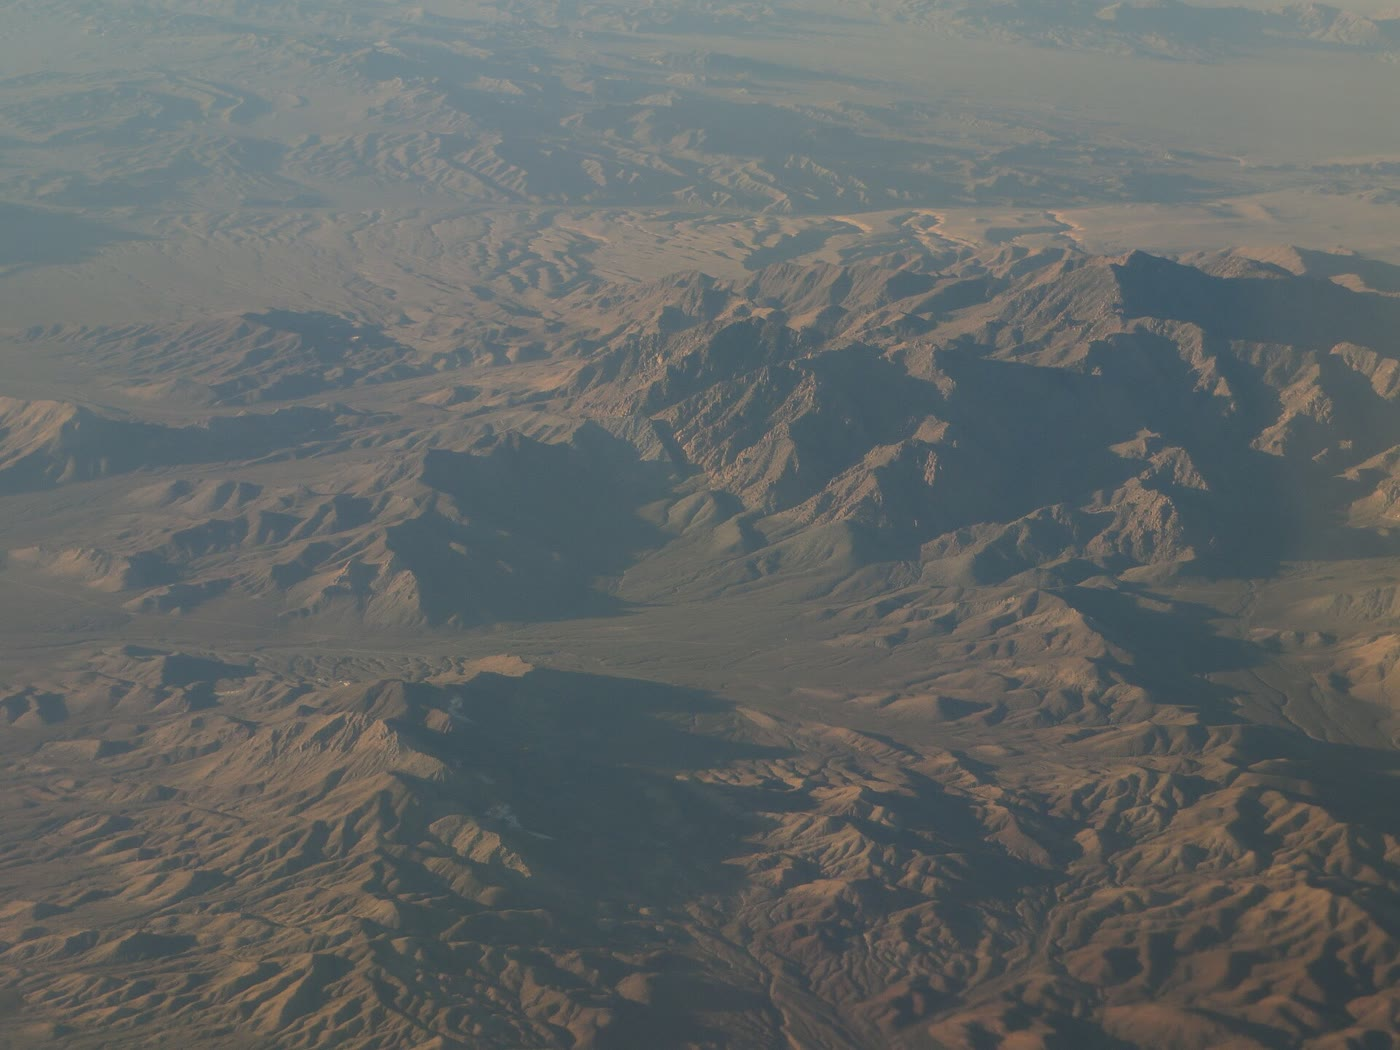
\includegraphics[width=\linewidth]{images/book5/b3-basin-and-range.jpg}

{\scriptsize طبوغرافيا الأحواض والسلاسل جنوب وادي الموت، كاليفورنيا،
من الجو: سلاسل متوازية من كتل صدعية مائلة تفصل بينها
أحواض مملوءة بالرواسب. الصورة: \mbox{\textdir TLT Ken Lund, CC BY-SA 2.0}.}
\end{minipage}
\end{inthefield}
% ledger: photo:b3-basin-and-range

\section{التمارين}

\begin{exercise}[$\star$]\label{exo:b3:extension-strike-slip:1}
نطاق من الكتل الدومينوية الصلبة تحوي صدوعًا تنحدر بزاوية \ang{35}؛ تكوّنت عند
\ang{50}. احسب انحدار الطبقات وعامل الاستطالة.
\end{exercise}

\begin{exercise}[$\star$]\label{exo:b3:extension-strike-slip:2}
بيّن ما إذا كانت كل خطوة تفتح حوضًا أو ترفع ظهرة: صدع أيمن
خطوته نحو اليمين؛ صدع أيمن خطوته نحو اليسار؛ صدع أيسر خطوته نحو
اليسار؛ صدع أيسر خطوته نحو اليمين.
\end{exercise}

\begin{exercise}[$\star$]\label{exo:b3:extension-strike-slip:3}
تحرّك الصدع الانزياحي للبحر الميّت \qty{105}{km} في نحو \qty{20}{Myr}.
احسب متوسط المعدّل بوحدة \unit{mm/yr} وقارنه مع \qty{6}{mm/yr}
المستعمَل في حوض البحر الميّت.
\end{exercise}

\begin{exercise}[$\star$]\label{exo:b3:extension-strike-slip:4}
في الجزء المركزي من مقاطعة الأحواض والسلاسل، تبلغ استطالة \qty{235}{km} نسبةً
\qty{200}{\percent}. احسب عرض المنطقة قبل الاستطالة وبعدها. أعِد الحساب نفسه
للجزء الشمالي عند \qty{50}{\percent}.
\end{exercise}

\begin{exercise}[$\star\star$]\label{exo:b3:extension-strike-slip:5}
تحرّك صدع سان أندرياس على الأقل \qty{563}{km} خلال فترة من 15 إلى
\qty{20}{Myr}. احسب مدى المتوسطات للمعدّلات، وقارنها بانجراف حالي
يبلغ نحو \qty{51}{mm/yr}. ما الذي يمكن أن يفسّر الفرق؟
\end{exercise}

\begin{exercise}[$\star\star$]\label{exo:b3:extension-strike-slip:6}
مع $\mu = 0.6$، احسب \omterm{def:b3:structural-analysis:palaeostress}{نسبة الإجهاد} $\sigma_1/\sigma_3$ اللازمة لانزلاق الصدوع
العادية المنحدرة بزوايا \ang{60}، \ang{50} و\ang{40}، وانحدار القفل.
\end{exercise}

\begin{exercise}[$\star\star$]\label{exo:b3:extension-strike-slip:7}
احسب انحدار القفل لصدع عادي عند $\mu = 0.4$ و$\mu = 0.2$.
ما معامل الاحتكاك الذي يسمح لصدع منحدر بزاوية \ang{15} بالانزلاق تحت
الإجهاد $\sigma_1$ الشاقولي؟
\end{exercise}

\begin{exercise}[$\star\star$]\label{exo:b3:extension-strike-slip:8}
في مقطع زلزالي موازٍ للانزلاق، للصدع اللستري إزاحة أفقية قدرها
\qty{2.5}{km}؛ ثم ينبسط إلى صدع انفصال عمقه \qty{4.0}{km}. احسب مساحة
المنخفض الواقع تحت القمة الأصلية للجدار المعلّق، وتحت طبقة
تقع أوّلًا على عمق \qty{1.5}{km}.
\end{exercise}

\begin{exercise}[$\star\star$]\label{exo:b3:extension-strike-slip:9}
يبلغ طول حوض البحر الميت \qty{132}{km}، وقد امتُدّ بعامل قدره 1.19
على طول محوره. احسب طوله الأوّلي والاستطالة، والزمن الذي تستغرقه
الاستطالة بمعدّل \qty{6}{mm/yr}.
\end{exercise}

\begin{exercise}[$\star\star\star$]\label{exo:b3:extension-strike-slip:10}
تدور كتل تفصل بينها مسافة \qty{3.0}{km}، مقيسةً عموديًا على صدوعها،
من انحدارات الصدوع \ang{60} إلى \ang{45}. احسب العرض الأفقي لكتلة واحدة
قبل الدوران وبعده، والاستطالة لكل كتلة، وانحدار الطبقات.
لماذا يجب أن تنحدر الطبقات في الاتجاه المعاكس لانحدار الصدوع؟
\end{exercise}

\begin{exercise}[$\star\star\star$]\label{exo:b3:extension-strike-slip:11}
أعطِ زوايا القصوص R و\mbox{\textdir TLT R$'$} وكسور الشدّ لصخر
ذي $\phi = \ang{40}$ في نطاق أيسر يمتدّ شرق--غرب،
وذلك بوصفها سمتيات، واذكر اتجاهات انزلاقها.
\end{exercise}

\begin{exercise}[$\star\star\star$]\label{exo:b3:extension-strike-slip:12}
تتشكّل منطقة من الدومينوات، وتكون صدوعها بأفضل انحدار للانزلاق،
ثم تدور حتى تنقفل. احسب أكبر عامل استطالة يُعطيه الدوران وحده
عند $\mu = 0.6$ وعند $\mu = 0.85$، وبيّن أيّ الصخور يمكن أن تُستطال
أكثر قبل أن تتشكّل صدوع جديدة.
\end{exercise}

\section{مسألة: حوض مِيرو نصف الغرابن}

\begin{problem}[{مسألة نهاية الأسبوع --- استطالة حافة صدع قاريّ متخيَّلة،
من دومينواتها وصدعها اللستري ولبّها المعقّد
وصدعها التحويلي}]
\label{pb:b3:extension-strike-slip:1}
% values: calc/ch09.py; domino_extension.py; rollover.py
حوض مِيرو نصف الغرابن حوضٌ متخيَّل على حافة
شقّ قاريّ. صدعه الرئيسي لستري، وينحدر بزاوية \ang{60} عند السطح.
في جداره المعلّق، تُقطع منطقةٌ عرضها \qty{24.0}{km} بصدوع مستوية تنحدر الآن
\ang{42} شرقًا، وتنحدر الطبقات بينها \ang{18} غربًا. في مقطع زلزالي
موازٍ للانزلاق، للصدع الرئيسي إزاحة أفقية قدرها \qty{3.2}{km}،
ويهبط أعلى جداره المعلّق دون مستواه الأصلي على مساحة قدرها
\qty{16.0}{km^2}. وعلى طول الامتداد نحو الجنوب، أزالت التعرية الصفيحة العليا
من النظام نفسه وكشفت عن معقّد لبّي. وإلى الشمال، يصل صدع تحويلي أيسر
نصف الغرابن بالذي يليه. خذ $\mu =
0.6$، و$g = \qty{9.8}{m/s^2}$، وكثافة قشرية قدرها
\qty{2800}{kg/m^3}.

\medskip\noindent\textbf{الجزء الأول --- الدومينوات.}
\begin{enumerate}
  \item لماذا يساوي الانحدار الأوّلي للصدوع مجموع انحداري الصدع الحالي
        والطبقة؟ أعطِه، وقارِنه بنظرية أندرسون.
  \item احسب عامل استطالة المنطقة.
  \item احسب عرضها الأوّلي والاستطالة التي تسجّلها.
  \item احسب النسبة $\sigma_1/\sigma_3$ اللازمة لانزلاق الصدوع الآن، وقارنها
        بنسبة صدوع جديدة مُحَسَّنة التوجيه.
  \item عند أيّ انحدار تنقفل هذه الصدوع، وما عامل الاستطالة الذي يمكن أن تبلغه
        المنطقة بالدوران وحده؟ ماذا يحدث عندئذ؟
\end{enumerate}

\medskip\noindent\textbf{الجزء الثاني --- الصدع الرئيسي اللستري.}
\begin{enumerate}[resume]
  \item اشرح، بإنشاء الإزاحة الأفقية الثابتة، لماذا تميل طبقات الجدار المعلّق
        نحو الصدع.
  \item احسب عمق \omterm{def:b3:extension-strike-slip:detachment}{صدع الانفصال}.
  \item تُعرف مساحة المنخفض بدقّة \qty{10}{\percent}. ما مدى
        دقّة معرفة العمق؟
  \item ما مساحة المنخفض التي تتنبّأ بها لطبقة كانت أوّلًا
        على عمق \qty{2.0}{km}؟
  \item ما الاستطالة الأفقية عبر الصدع الرئيسي؟
  \item كيف تسجّل رسوبيات نصف الغرابن نشاط
        الصدع؟
\end{enumerate}

\medskip\noindent\textbf{الجزء الثالث --- المعقّد اللبّي.}
\begin{enumerate}[resume]
  \item توازنت ميلونيتات الجدار المرتكز عند \qty{5.5}{kbar}. احسب
        عمقها.
  \item أُغلقت ميكاها على الأرغون عند \qty{24}{Ma}،
        وتظهر حصى من الميلونيتات نفسها في ردم نصف الغرابن عند \qty{16}{Ma}.
        احسب متوسط معدّل الاستخراج، آخذًا عمق الإغلاق
        عمقَ السؤال السابق.
  \item لإصعاد الميلونيتات، كم يلزم من الانزلاق على صدع انفصال متوسط
        انحداره \ang{30}، وكم من الاستطالة الأفقية؟
  \item ينحدر \omterm{def:b3:extension-strike-slip:detachment}{صدع الانفصال} \ang{15} عند السطح اليوم. هل كان يمكن أن ينزلق بذلك
        الانحدار تحت $\sigma_1$ شاقولي؟ أعطِ طريقتين للخروج من ذلك.
  \item إذا انزلق بزاوية \ang{45} في العمق، فبأيّ زاوية دار الجزء المكشوف،
        ولماذا؟
  \item قارن استطالة المعقّد اللبّي
        باستطالة نصف الغرابن.
\end{enumerate}

\medskip\noindent\textbf{الجزء الرابع --- الصدع التحويلي.}
\begin{enumerate}[resume]
  \item يتخطّى الصدع التحويلي الأيسر إلى اليسار بمقدار \qty{4.0}{km}، وتتداخل
        فرعاه على امتداد \qty{3.0}{km}. هل يفتح التخطّي حوضًا
        أم يرفع حافة؟
  \item انزلق الصدع بمعدّل \qty{5}{mm/yr} طوال \qty{1.2}{Myr}. احسب
        الإزاحة.
  \item احسب المساحة المفتوحة، وطول قاع الحوض (التداخل مع الإزاحة)،
        ونسبة طوله إلى عرضه.
  \item قارن هذه النسبة بنسبة حوض البحر الميت، الذي طوله \qty{132}{km}
        وعرضه من 7 إلى \qty{10}{km}.
  \item حيث ينحني الصدع نفسه في الاتجاه الآخر، ما البنية التي تتشكّل،
        وماذا يُظهر مقطع عرضي عبرها؟
  \item ما الاستطالة الأفقية الكلية عبر حوض مِيرو نصف الغرابن، من صدعه
        الرئيسي ودومينواته؟
\end{enumerate}
\end{problem}
